\section{Wireless Data Transfer}\label{sec:datatrans}
This section describes the most important point for the research. If the data is not transferred wireless to the external system, the exoskeleton will not be monitored as a wired connection will impede the exoskeletons movement ability. In section \ref{sec:orgmod} the original architecture model is described. In section \ref{sec:impmod} the improved model is described that came forth from the limitations of the original model.

\subsection{Original model} \label{sec:orgmod}
EtherCAT is already used on the exoskeleton as stated in section \ref{sec:etherCat}. This lead to the first point, whether the current EtherCAT-configuration could be extended. The exoskeleton (E) and the receiver (R) would both be running Simulink. The receiver would then process the data and send it to the interface (I). This leaves the possibility to  extend to multiple interfaces, by putting a broadcaster (B) between the receiver and the interface(s). A visual representation of this model can be found in figure \ref{fig:catmodel}. However, the EtherCAT-blocks in Matlab \cite{web:ethercat} do not support wireless connections. Therefore it is not possible to implement this solution.

The next step was to check whether the original model would work using the Ethernet-blocks \cite{web:ethernet} instead. The original model would only need a slight change, which results in figure \ref{fig:netmodel}. However, after consulting with someone from Speedgoat GmbH, this model was deemed as not preferred. If a USB wireless adapter would be used, drivers would need to be written for it as Simulink cannot use the standard drivers.

When examining the time frame for delivering the various product parts, it was deemed more practical to use a networking solution which requires less time and effort to implement, and spend more time and focus on building the user interface.

\begin{figure}[H]
	\centering
	\begin{minipage}{.49\textwidth}
		\centering
		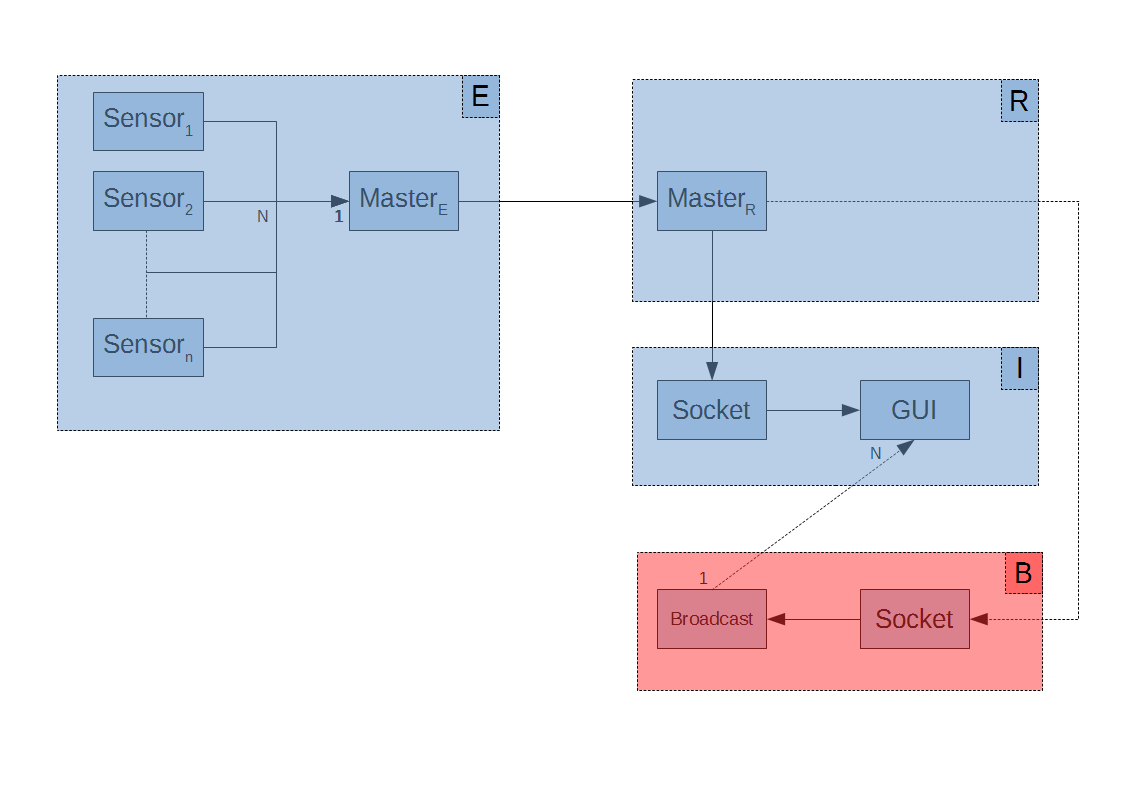
\includegraphics[width=\linewidth]{ERBI-Model-EtherCat}
		\subcaption{EtherCAT variation}
		\label{fig:catmodel}
	\end{minipage}
	\rulesep
	\begin{minipage}{.49\textwidth}
		\centering
		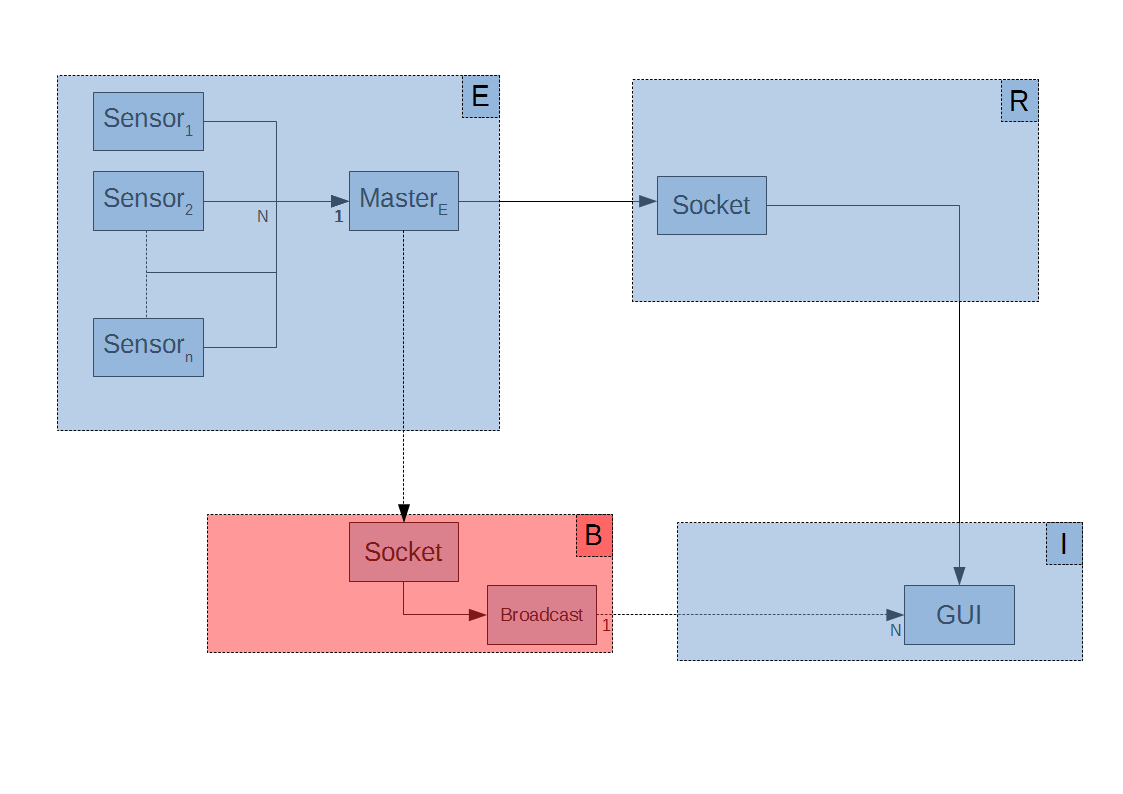
\includegraphics[width=\linewidth]{ERBI-Model-TCP}
		\subcaption{Ethernet variation}
		\label{fig:netmodel}
	\end{minipage}
	\caption{The variations of the original model}
	\label{fig:firstmodel}
\end{figure}

\subsection{Improved models} \label{sec:impmod}
Due to a lack of options to add wireless communication directly to the Speedgoat, bridging hardware is required to attach a wireless card on a wired interface on the Speedgoat. An abstract visualisation of this can be found in figure \ref{fig:improvedmodel}. The following models are based on the possibility to build a wireless connection via such a device. In all variants, this device will be configured as a wireless access point to which clients can connect.
The proposed device for acting as a wireless bridge between the Speedgoat and the client is a Raspberry Pi 3. This board has both an ethernet port for connecting the Speedgoat and a wireless chip capable of running in accesspoint mode. On top of that, experience within the team of setting up networks with a Raspberry Pi is present.

\subsubsection{Transparant Bridge Model}\label{sec:tbm}
This model requires the wireless bridge to transparently bridge the wired and wireless connections on the network level. This makes direct communication between the data provider (E) and client (I) possible. The Simulink model on the exoskeleton can directly send acquired data to a client with a GUI build in Matlab. By using Matlab to build the GUI we can make use of the extensive data visualization features and data processing features of Matlab without the need of translating this data for use with another program. 

Although the chosen networking model does not differentiate between networking protocols, UDP send \cite{web:UDPSend} is considered as a good choice due to the ease of setting up non-blocking communication.

\subsubsection{Listening Bridge Model}\label{sec:lbm}
Like the previous model, this solution comprises of a data provider in Simulink running on the exoskeleton and a Matlab client, however the networking model is slightly different. Instead of building a transparent connection bridge, the wireless bridge will run software listening for connections both on the wireless and wired network connection. This will eliminate the need to use server sockets on the exoskeleton and on the client, instead both of them will build a connection to the bridge. The software running on the bridge will ensure that data pushed from the exoskeleton will be pushed further to any connected client.

\subsubsection{Standalone Model}\label{sec:sm}
The Standalone Model with a non-Matlab executable running on the client can make use of the previous two networking models. However, if the solution similar to section \ref{sec:lbm} is chosen, the bridge might be used as a data processing unit as well. The advantage of this is that the data can be transformed to a format that eases processing on the client.

\subsubsection{Webservice Model}\label{sec:wm}
The Webservice Model avoids the need of running a standalone executable or the need of a Matlab installation on the system running the client. The client connects to the network, and the full interface can be opened in a web browser by pointing the location to the url of the bridge. This will require data processing on the bridge, as it has to reformat the data send by Simulink on the exoskeleton to a format suitable for sending over a WebSocket to the client. The client can not use a technique like polling because of the need for real-time data.

\begin{figure}[h]
	\centering
	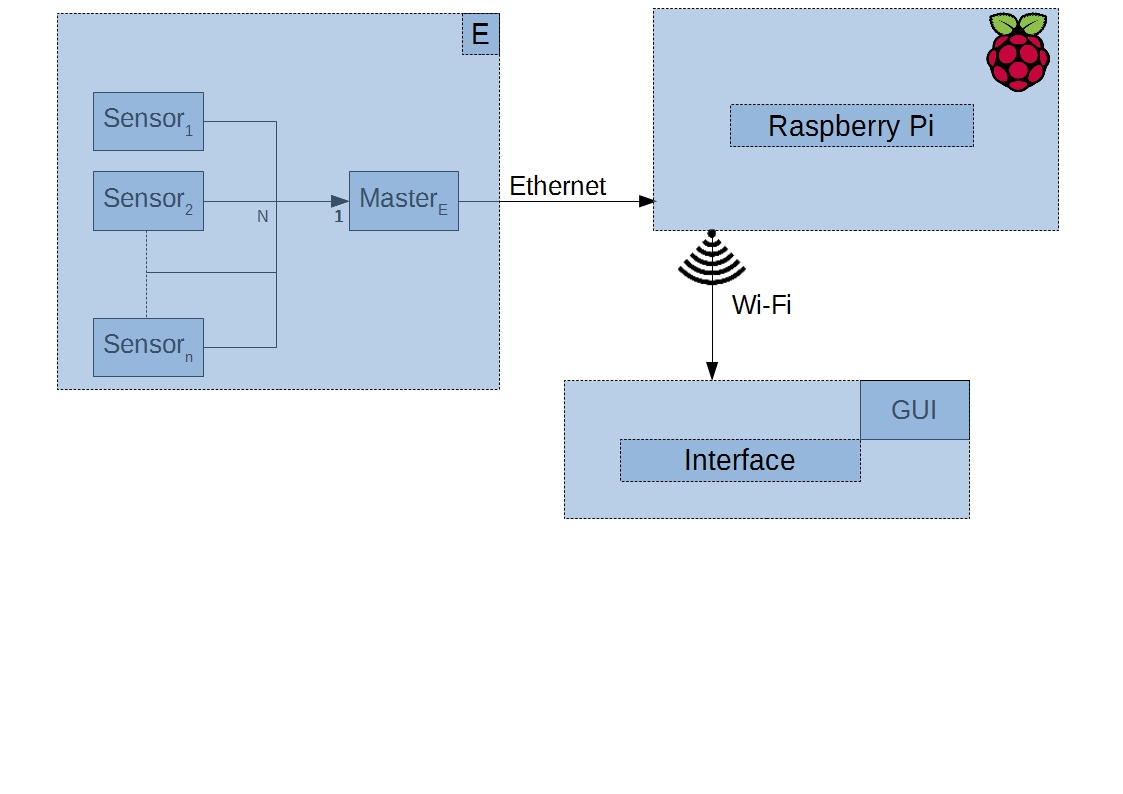
\includegraphics[width=.75\textwidth]{ERBI-Model-RaspPie}
	\caption{Abstract version of the improved model} 
	\label{fig:improvedmodel}
\end{figure} 
